\section{Fallstudie}
In diesem Kapitel erfolgt die Beschreibung der technischen Realisierung dieser Fallstudie. Dabei werden die verwendeten Technologien als auch die eintretenden Szenarien und deren Verarbeitung beschrieben.

\subsection{Verwendete Technologien}
Damit die Fallstudie in einer angemessenen Art präsentiert werden kann, erfolgt die Realisierung des Projekts als Web-Applikation. Dafür wird mit \textit{Spring-Boot} ein quelloffenes Java-Framework verwendet. Darin enthaltene Komponenten wie \textit{SpringMVC} und der Applikation-Server \textit{Tomcat} ermöglichen eine konfigurationsarme Erstellung der Webanwendung. Die Webanwendung besteht im Wesentlichen aus einer serverseitigen (Backend) und einer clientseitigen (Frontend) Komponente. \linebreak
Das Backend folgt dem Architekturmuster Model-View-Controller. Die Controller-Klassen enthalten REST-Schnittstellen, durch die es möglich ist, einzelne Events zu senden und diese durch eine Complex Event Processing - Engine zu verarbeiten.\linebreak 
Das Frontend wird durch Verwendung der \textit{Java Server Pages} - Technologie (JSP) in Kombination mit der \textit{Java Standard Tag Library} (JSTL) umgesetzt. Diese ermöglicht die Visualisierung des aktuellen Zustands des Straßenausschnitts, die Steuerung von Eventströmen und das Auslösen einzelner Events. Die Kommunikation zwischen Front- und Backend erfolgt durch den Einsatz von \textit{Asynchrounous JavaScript and XML} (AJAX) statt. \linebreak
Als Complex Event Processing - Engine wird \textit{Esper} verwendet. Esper ermöglicht die schnelle Verarbeitung großer Mengen eingehender Nachrichten und ist somit sehr gut für die Verwendung in Smart Traffic Szenarien geeignet. 

\subsection{Beschreibung der Ausgangslage}
Das Szenario dieser Fallstudie beschreibt den fiktiven Kartenausschnitt aus Abb.\ref{fig2}. Dieser Ausschnitt besteht aus den drei Kreuzungen K1, K2 und K3, einer Nord-Süd-Achse S3 und einer West-Ost-Achse S1 als Hauptverkehrsstraßen sowie einer Bahnlinie mit Bahnübergang an der West-Ost-Achse. Die Verkehrsteilnehmer sind autonom fahrende (Einsatz-)Fahrzeuge, deren Fahrtrichtung durch Pfeile in den Tabellen auf Abb.\ref{fig2} dargestellt werden. Als Ausweichrouten können die parallel verlaufende nördliche Straße S2 sowie die westlich von der S3 verlaufende S4 befahren werden. Diese werden verwendet, wenn es die Verkehrslage durch eines oder mehrere der möglichen nachfolgend aufgelisteten Szenarien erfordert.

\begin{itemize} 
\item Unfall an Kreuzung K2
\item Geschlossene Bahnschranke
\item Erhöhte Stickstoffbelastung an Kreuzung K2
\item Überhöhtes Verkehrsaufkommen an Straße S1
\end{itemize}

\begin{figure}[ht]
	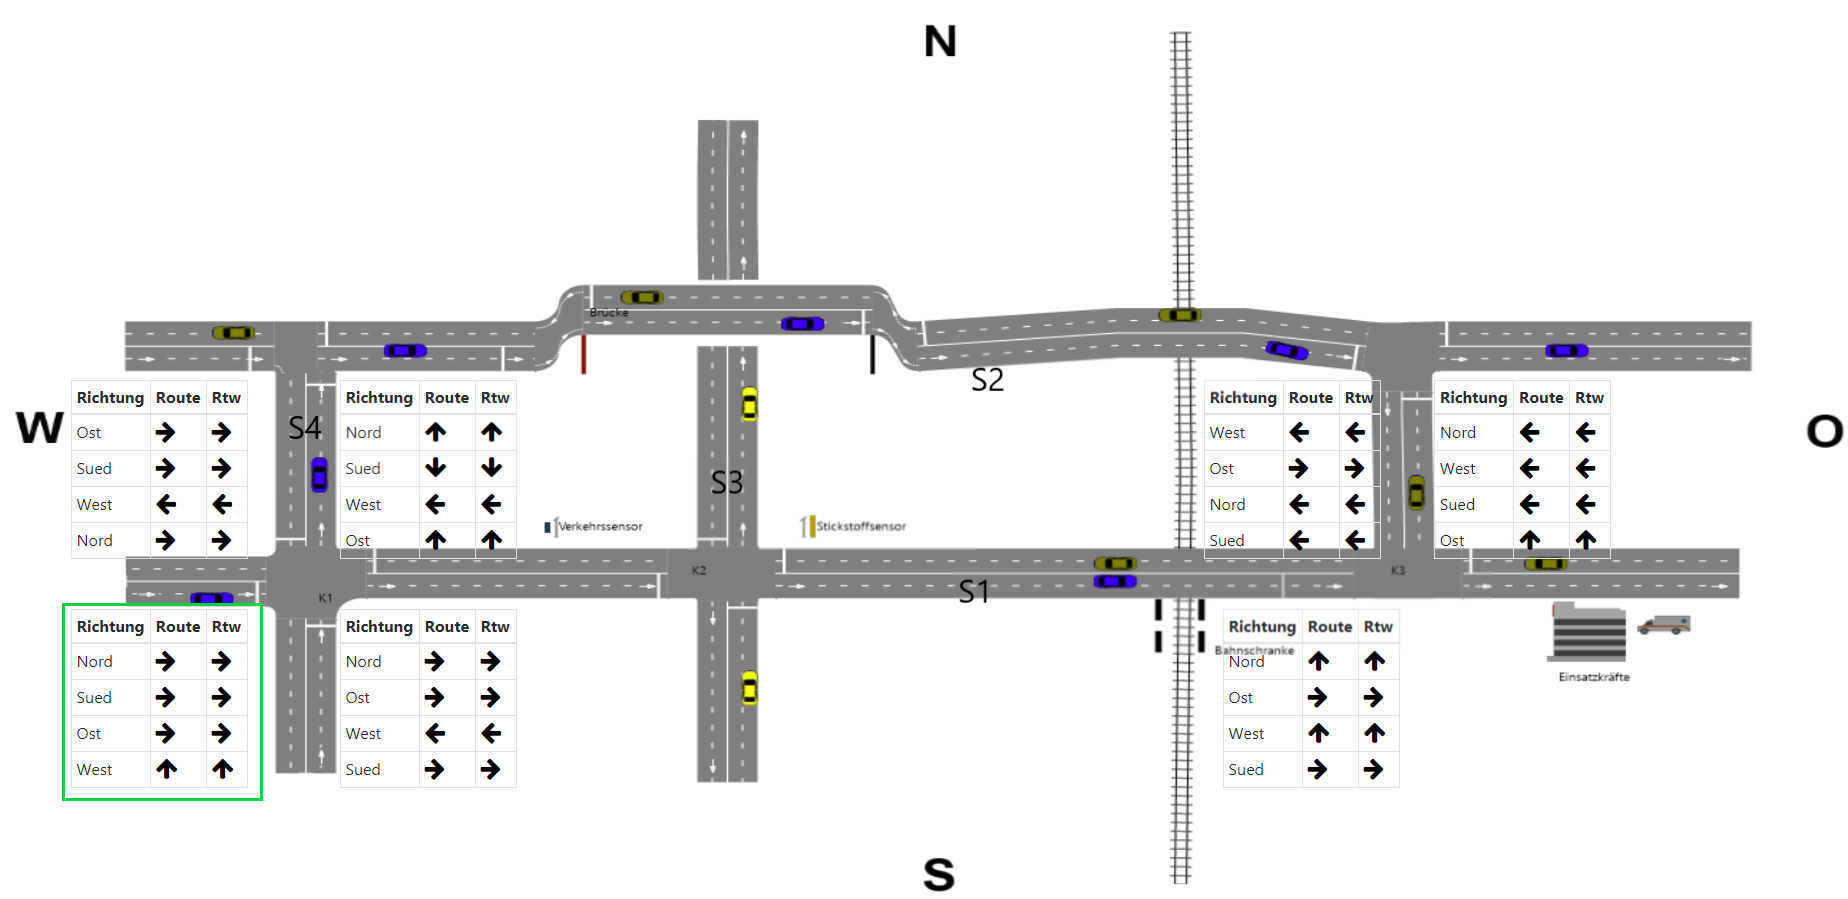
\includegraphics[width=\textwidth]{images/dataanalyticswebapp.png}
	\caption{Straßenausschnitt mit Anzeige der Fahrrichtung}
	\label{fig2}
\end{figure}

\subsection{Unfall an Kreuzung K2}
\subsection{Geschlossene Bahnschranke}
\subsection{Erhöhte Stickstoffbelastung an Kreuzung K2}
\subsection{Überhöhtes Verkehrsaufkommen an Straße S1}

\clearpage
